
\chapter{Introduction} \label{intro}


The emergence of social media coupled with big data methodology has opened the door for the next generation of surveillance systems. We develop methods to create such systems on the popular social network, Twitter. We have found \cite{www2013} issues with previous approaches to use Internet data for disease surveillance (for example, \cite{gft,culotta2010towards,culotta2013lightweight,signorini2011use}). First, these systems have been shown to perform poorly \cite{www2013,butler2013google,copeland2013google,lazer2014twitter,lazer2014google}. Second, these systems tend to not use or generate in depth knowledge about the disease. Third, these systems do not provide information on how to influence activity related to the disease. Here, we provide a further discussion of these issues and present ways in which they can be addressed.

\section{Issues with Current Approaches towards Digital Epidemiology}
\subsection{Lack of Validation}
Google Flu Trends (GFT)--a real time influenza surveillance system based on Google searches--is generally considered the baseline for web-based disease surveillance \cite{gft}. However, GFT has been shown to perform poorly at times, its most `famous' gaft being the January 2013 overestimate of more than twice the true level of influenza prevalence \cite{butler2013google,copeland2013google,lazer2014google}. One explanation for this overestimate provided by the Google Flu Trends team \cite{copeland2013google} and others \cite{butler2013google,lazer2014google} is that a particularly strong public interest in the disease  confused the system. This interest was due in part to a feedback loop caused by GFT's high estimates. Google has since modified their algorithm to dampen these types of events\cite{copeland2013google}, but Lazer et al. \cite{lazer2014google} have argued that this both doesn't fix the issue and further obfuscates the model.

Another issue of concern is the difficulty in model comparison. For example, the original GFT paper was published in 2008 \cite{gft} and finds a mean correlation of \(0.9\) while Signorini et al. \cite{signorini2011use} report their model as having an average absolute error of \(0.28\%\) on the 2009-2010 flu season\footnote{The reader should also note that the average flu rate during this period was approximately \(3.9\%\), resulting in a relative error of about \(0.28/3.9 = 7.2\%\).}. However, when we attempt to standardize these two paper's methods on Twitter data from the 2011-2012 flu season \cite{www2013}, we find the Google's model has a mean correlation of \(0.88\) and Signorini's model has a mean correlation of \(0.76\) (mean absolute error = \(5.7\%\)). Additionally, one of Culotta's \cite{culotta2010towards} models (``simple-freq-corr'') was found to have a correlation of \(0.65\) in our dataset compared to his finding of a correlation of \(-0.034\), providing a rare counter example of publication bias. This general lack of reproducibility of results, besides GFT's results, is not due to fraud or incorrect implementation, but due to some of these models showing a high sensitivity to the initial data---resulting in a questionable efficacy of comparing different models. 

\subsection{Lack of Semantic Knowledge}

\begin{figure}
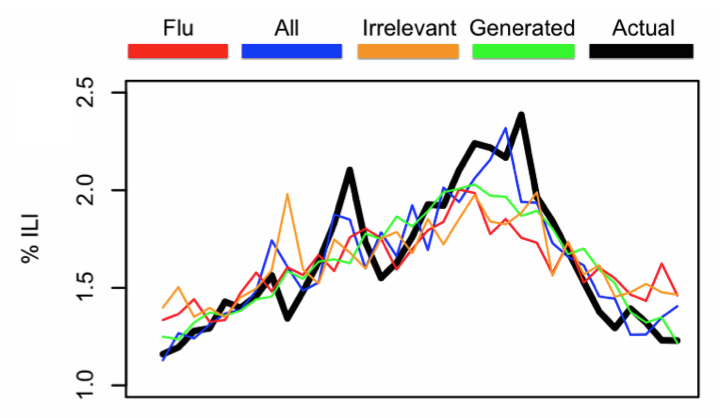
\includegraphics{introduction/figures/www2013_svmr.png}
\caption[SVM-regression for the 2011-2012 Influenza season using multiple datasets.]{SVM-regression for the 2011-2012 Influenza season using multiple datasets, from \cite{www2013}.}
\label{fig:intro_www2013}
\end{figure}


As mentioned above, GFT does not specifically differentiate between searches about \emph{having} influenza and \emph{news} about influenza. A similar issue occurs with Twitter analysis: rate limiting makes it impossible for a third party to gain \emph{all} tweets during a period of time. This is commonly addressed by searching for Tweets which contain keywords such as ``flu'' or symptoms of influenza. Note that this does not filter out Tweets about news about influenza, although work has been done in filtering out these messages \cite{culotta2010towards,lamb2013separating}. However, the bag-of-words approach for Twitter disease modeling has one major issue: we've been able to replicate the results from datasets based on flu keywords by using tweets that were collected using completely irrelevant search terms, specifically keywords related to zombies (see Figure \ref{fig:intro_www2013}).

Additionally, we've compared an unfiltered, random sample of tweets and generated time varying frequencies simply by 
\begin{equation}
x_{i,t} = (sin(t*\alpha_{i,1} + \alpha_{i,0})+\mathcal{N}(0,.1))/1000 + .001
\end{equation}
where \(\alpha_{i,0}\) and \(\alpha_{i,1}\) are randomly generated weights, \(\mathcal{N}(0,.1)\) is a normally distributed random variable with standard deviation of 0.1 and \(x_{i,t}\) is the value of curve \(i\) at time \(t\). While this is essentially building a model based simply off of the initial, disease frequency's time series, the fact that its performance is equivalent to more complex, data mining approaches brings the value of the later approaches into question. Further discussion and methods are available in chapter \ref{www2013}.

Besides human determined keywords, all papers surveyed do not encode any semantic knowledge into their models which may be one explanation for issues related to model generalization outside of the initial dataset.


\subsection{Obsession with Disease Tracking over Knowledge Generation}

Infectious disease studies using big data have strongly focused on surveillance systems \cite{world2006communicable} to either predict the future or current state of a disease's spread. \cite{gft,chunara2012new,culotta2010towards,goel2010predicting,signorini2011use,kim2013use} These models tend to strongly correlate with the actual disease's prevalence (for example, Yaari et al. \cite{yaari2013modelling} report \( r > .97\)) limiting the value of further optimizing these methods or the likelihood that improvements will be statistically significant. Other topics--such as disease transmission\cite{salathe2010high,Cauchemez:2011cp,Ferrari:2011ht}, the use of vaccines\cite{Salathe:2011gr,Wells:2013tp,Seale:2010br,Larson:2013kh,Bansal:2006di,Salathe:2008ct}, disease movement patterns\cite{Huang:2013ed,Balcan:2009ub,Afzal:2011bc}, behavioral effects of diseases\cite{Funk:2010cc,Jones:2009cv,Funk:2009ks} or the economic impact of diseases\cite{Tudor:2008kh,GruneYanoff:2011hl,Glasser:2004is}--are widely studied topics in traditional epidemiology, but have been neglected when it comes to big data analytics. This is particularly odd considering that the basis for these other topics, measurements of a population's illness, are also the basis for disease surveillance systems.

%While the WHO's definition of a surveillance system  includes ``response and control'' of a disease, it is unclear if providing real-time surveillance is much better than the CDC's current ILINet, which has a lag of 1 to 2 weeks. Instead, predictive models and work on designing influential messages about a disease may be more effective. Very little work has been put in to predicting future disease rates, possibly due to a much higher difficulty compared to models which  ``predict the present'' rate of disease. \cite{gft,chunara2012new,culotta2010towards,goel2010predicting,signorini2011use} Indeed, one of the few papers to attempt such a model ``demonstrated the inability of the prediction to follow the initial rise of the ILI data.''\cite{kim2013use} The issues regarding response and controll have been covered in part by advertising research, although more work on Tweets and messages specific to disease is needed \cite{timimi2013shape}.


\subsection{Inability to Influence Disease}

Using messages to influence behavior is a well studied technique,\cite{Eyssartier:2008jy,CavalliSforza:1982we,Rendell:2010go,Traulsen:2010ja,Centola:2010ki,Bond:2012ff} indeed it is the basis of the advertisement industry. However, work on public health messages has lagged more commercial topics \cite{timimi2013shape}. Work has generally focused on an individual's knowledge about a disease, as discerned through surveys\cite{Jones:2009cv} or a simple analysis of events\cite{Kinsman:2012wi}. While an understanding of the population's opinion on a topic can be the basis for crafting an influential message, it is a relatively primitive approach compared to large scale A/B testing \cite{bakshy2014www} or modeling a user's behavior using hundreds of thousands of variables. \cite{mcmahan2013ad}

\section{Proposed Solutions}
\subsection{On the ground validation through professional diagnoses}
\label{subsec:intro_uhs}
Others have worked on a top-down approach by using region-wide disease prevalence data from which Twitter data can be fit. \cite{gft,culotta2010towards,culotta2013lightweight,signorini2011use} However, they do not aim to say whether a specific Twitter user is ill, limiting the usefulness of such methods. In chapter \ref{www2014}, we consider a bottom-up approach to disease surveillance by diagnosing users based off of their Twitter information \cite{www2014}. To do this, we survey 104 people that were \emph{professionally} diagnosed with influenza through Penn State's University Health Services. As a control group, we survey an additional 122 individuals that were \emph{not} diagnosed with influenza. From this data, we were able to collect Twitter data from 104 users.

%To match other work, we started by considering Tweets that were filtered by keywords that a domain expert may choose: ``flu,'' ``influenza,'' ``sick,'' ``cough,'' ``cold,'' ``medicine'' and ``fever.'' While five of the keywords did provide some information, models based simply on these keywords did not perform well (see Figure \ref{fig:intro_www2014}, orange curve). Additionally, ``influenza'' appeared only once and was not in the context of the poster being ill. Thus, search terms that previous work \cite{culotta2010towards,signorini2011use} has considered useful does not seem to be very useful. 


%We also looked for user's that specifically said that they were sick with influenza-like symptoms. We hand rated all tweets during times when the users were sick, according to their medical records, and hand rated a subset of all other Tweets as a control. We found that half (\(17/35 \approx 48.6\%\)) of the users specifically mentioned their illness and we didn't find any users mentioning their influenza-like-illness in the control set. A significant signal, but we needed to find more for a true diagnostic system.

We employed machine learning algorithms such as naive Bayes and support vector machines to use the aggregated set of messages a user posted during the time that she was ill, or an equivalent aggregation when she was healthy, to attempt a diagnosis. Next we looked at non-message information. We performed anomaly detection on a user's rate of Tweeting to see if their usage changes when sick. We find a significant difference in activity, however the results are too noisy to be considered a viable method to diagnose influenza. We consider the aggregated messages from a user's friends \emph{followers} and perform text analysis on them, as was done on the user's messages. We find that a user's follows are a much stronger signal toward a user's health than the accounts that a user follows. This hints at the Twitter's network structure: I follow both celebrities and my friends, but only my friends follow me. Finally, we employ meta-classifiers which use the output of each of the previous classifiers discussed as an input for a final classifier to get better classifier accuracies.



%\begin{figure}
%\centering
%\begin{subfigure}{.3\textwidth}
%  \centering
% \includegraphics[width=.95\linewidth]{figures/measure/uhs_graph.png}
%\end{subfigure}
%\begin{subfigure}{.3\textwidth}
%  \centering
%  \includegraphics[width=.95\linewidth]{figures/measure/uhs_graph_with_others_with_singleton.png}
%\end{subfigure}
%\begin{subfigure}{.3\textwidth}
%  \centering
%  \includegraphics[width=.95\linewidth]{figures/measure/uhs_graph_with_others_no_singleton.png}
%\end{subfigure}
%\caption{The difference in scale between our network of users with professional diagnoses (left), and the network that is generated when their friends and followers are included (center) illustrates the value of employing less accurate data sources. By removing nodes with degree less than two (right) additional typology is visible.}
%\label{fig:measure_mininetwork_full}
%\end{figure}

\section{Quantifying Disease Dynamics}
In chapter \ref{longitude}, we combine this classifier with a dataset of 2.7 billion Tweets to track 16 million users' disease states over a period of four years. Additionally, we employ geographical analysis of the users' supplied location information to approximate his real-world social network, \cite{hawelka2014geo,leetaru2013mapping,tatem2014mapping} specifically with respect to disease, which has previously been approached through measuring real world contacts. \cite{isella2011close,salathe2010high,smieszek2014should} We do this by seeing if other users near a given user can inform us about the given user's future health status. That is, are they likely to get sick when people near them have recently been sick?

This question can be answered based on probabilities, but instead we decide to model it based on the base reproduction rate, \(R_0\). This rate is the basis of most disease spread models, however, it is generally calculated by fitting curves to measured disease prevalence rates.\cite{yang2015inference} Attempts to study peer to peer transmission are limited in size (generally by the costs of tracking a group's disease states) to either 10's or 100's of individuals\cite{Cauchemez:2011cp,moser1979outbreak,klontz1989outbreak,salathe2010high}. Instead, we exploit an already developed social network platform, Twitter, as the basis of our collection, allowing us to preform these studies at web-scale.

%We consider using this data and classifier to add to work about whether or not a user's network on Twitter can be used to approximate his real-world social network, \cite{hawelka2014geo,leetaru2013mapping,tatem2014mapping} specifically with respect to disease, which has previously been approached through measuring real world contacts. \cite{isella2011close,salathe2010high,smieszek2014should} We do this by seeing if a user's friends' and followers' health statuses can inform us about the user's own health. That is, are they likely to get sick when their friends on Twitter are sick? Optimally, we would just use the accounts on which we have a professional diagnosis, but it appears that there is not enough data. Only 30 accounts share direct links between each other. Thus, we will also use the 913,082 accounts that either follow or are followed by our gold-standard users (for a visual representation of the difference in scale, see Figure \ref{fig:measure_mininetwork_full}). These users can be diagnosed by applying the methods described above.

\section{Targeting Messages towards Disease Related Individuals}

In chapter \ref{retweets}, we consider the effects of various aspects of a message on retweeting rates, a signal for reader interest.\cite{Suh:2010uw,Kim2012retweet,Stieglitz2012politics,gransee2012} We consider network structure, the type of user that posted a message and the textual content of the message. Additionally, sentiment analysis is often used to measure how positive or negative a message is.\cite{Kim2012retweet,Stieglitz2012politics,Zhao:2012vz,Bollen:2011wv,Ofek:ug} Again, this has been shown to be a signal for retweeting rates. However, in the case of disease information, messages tend to be predominately negative. Instead, we develop a model based on four dimensions of emotional content\cite{russell1977evidence,plutchik2001nature,Cambria2011} and apply it towards the retweet prediction problem.